% !TEX TS-program = pdflatexmk

\documentclass[14pt]{beamer}
\usepackage{newtxtext,newtxmath}
\usepackage{microtype}
\usepackage[english]{babel}
\usepackage{hyperref}
\usepackage{graphicx}
\usepackage{listings}
\lstloadlanguages{Python}
\lstset{language=Python}
\lstset{%
basicstyle=\ttfamily\bfseries,
keywordstyle=\color{blue}, emph={self}, emphstyle={\color{blue}},
identifierstyle=,
commentstyle=\color{brown},
stringstyle=\color{green!50!black},
showstringspaces=false,
emphstyle={[2]\color{purple}},
}
\usepackage{tikz}
\usepackage{pgfplots}
\usepackage{forest}
\usetikzlibrary{calc}
\usetikzlibrary{shapes}
\usetikzlibrary{positioning}
\usetikzlibrary{arrows}
\usepackage{array}
\newcolumntype{L}[1]{>{\raggedright\let\newline\\\arraybackslash\hspace{0pt}}m{#1}}

\mode<presentation>{
\usetheme{Madrid}
\definecolor{uabgreen}{cmyk}{.89,.31,.78,.17}
\usecolortheme[named=uabgreen]{structure}
\setbeamertemplate{navigation symbols}{}
\setbeamertemplate{footline}[frame number]
\setbeamertemplate{section in toc}[square]
\setbeamertemplate{subsection in toc}[square]
\setbeamertemplate{items}[square]
\setbeamercovered{transparent=5}
}

\newcommand{\keyword}[1]{{\color{blue}#1}}
\newcommand{\cmnt}[1]{{\color{gray}#1}}
\newcommand{\str}[1]{{\color{green!50!black}#1}}
\newcommand{\num}[1]{{\color{green!55!blue}#1}}
\newcommand{\defn}[1]{{\color{purple}#1}}

\newcommand{\limpl}{\Rightarrow}
\newcommand{\liff}{\Leftrightarrow}

\newcommand{\tab}{\hspace{1em}}

\author[Dr. Bethard]{Dr. Steven Bethard}
\institute[UAB CIS]{%
Computer and Information Sciences\\
University of Alabama at Birmingham}

\AtBeginSection[]
{
  \begin{frame}<beamer>{Outline}
    \tableofcontents[currentsection]
  \end{frame}
}

\tikzset{
  invisible/.style={opacity=0,text opacity=0},
  text visible on/.code={%
    \alt<#1>{}{\pgfkeysalso{text opacity=0}}
  },
  visible on/.code={%
    \alt<#1>{}{\pgfkeysalso{invisible}}
  },
  filled on/.code={%
    \alt<#1>{\pgfkeysalso{fill=gray}}{}
  },
  alt/.code n args={3}{%
    \alt<#1>{\pgfkeysalso{#2}}{\pgfkeysalso{#3}}
  },
}
\forestset{
  edge weight/.style={
    edge label={node[midway,above,sloped]{#1}}},
  invisible/.style={
    /tikz/invisible,
    edge={/tikz/invisible}},
  visible on filled on/.code n args={2}{%
    \alt<#1>{\alt<#2>{\pgfkeysalso{fill=gray}}{}}{\pgfkeysalso{invisible}}
  },
  visible on/.code={%
    \alt<#1>{}{\pgfkeysalso{invisible}}
  },
}

\newlength{\wumpusgridsize}
\newenvironment{wumpusgrid}[2]{%
\setlength{\wumpusgridsize}{#2}
\begin{tikzpicture}
\draw[very thick,step=\wumpusgridsize] (0,0) grid (#1\wumpusgridsize, #1\wumpusgridsize);
}{%
\end{tikzpicture}
}
\newcommand{\wumpustop}[5][]{%
\only<#2>{\node[#1] at (#3\wumpusgridsize+0.5\wumpusgridsize,#4\wumpusgridsize+0.75\wumpusgridsize) {#5};}
}
\newcommand{\wumpusbottom}[5][]{%
\only<#2>{\node[#1] at (#3\wumpusgridsize+0.5\wumpusgridsize,#4\wumpusgridsize+0.25\wumpusgridsize) {#5};}
}
\newcommand{\wumpusagent}[3]{\wumpusbottom{#1}{#2}{#3}{\fbox{A}}}
\newcommand{\wumpuspercept}[4]{%
\only<#1>{\node[red,inner sep=0pt] at (#2\wumpusgridsize+0.25\wumpusgridsize,#3\wumpusgridsize+0.75\wumpusgridsize) {\textbf{#4}};}
}
\newcommand{\wumpusknowledge}[4]{%
\only<#1>{\node[draw,cloud,inner sep=0pt,text width=1em,align=center] at (#2\wumpusgridsize+0.75\wumpusgridsize,#3\wumpusgridsize+0.75\wumpusgridsize) {\footnotesize #4};}
}


\title{Learning from Examples}
\date[]{20 Mar 2014}

\begin{document}


\begin{frame}
  \titlepage
\end{frame}

\section{Supervised Learning}

\subsection{Hypothesis Functions}

\begin{frame}{Supervised Learning}
\begin{block}{Key Ideas}
\begin{itemize}
\item Examine pairs of inputs and outputs
\item Guess a possible function mapping input to output
\item Predict outputs given new inputs
\end{itemize}
\end{block}
\bigskip
\begin{columns}
\begin{column}<2->{0.25\textwidth}
$
\begin{array}{lll}
f(1) & = & 1 \\
f(2) & = & 4 \\
f(3) & = & 9 \\
f(4) & = & 16 \\
f(5) & = & \alt<3->{\alert{25}}{?} \\
\end{array}
$
\end{column}
\begin{column}<4->{0.7\textwidth}
\begin{tabular}{lll}
$f$(Romeo and Juliet) & = & Shakespeare \\
$f$(Tom Sawyer)       & = & Twain \\
$f$(Macbeth)          & = & Shakespeare \\
$f$(Huckleberry Finn) & = & Twain \\
$f$(Othello)          & = & \alt<5->{\alert{Shakespeare}}{?} \\
\end{tabular}
\end{column}
\end{columns}
\end{frame}

\begin{frame}{Supervised Learning Components}
\begin{block}{Original Function}
An unknown function $f\!: D_f \rightarrow R_f$
\end{block}
\pause
\begin{block}{Training Examples}
Pairs of $(x, f(x))$ where $x \in D_f$ and $f(x) \in R_f$
\end{block}
\pause
\begin{block}{Hypothesis Function}
Some function $h\!: D_f \rightarrow R_f$
\end{block}
\pause
\begin{block}{Learning Goal}
Pick a hypothesis $h$ as close to $f$ as possible
\end{block}
\end{frame}

\begin{frame}{Problem Formulation}
\begin{block}{Defining a Machine Learning Problem}
Describe the function $f\!: D_f \rightarrow R_f$
\begin{itemize}
\item What is $D_f$?
\item What is $R_f$?
\end{itemize}
\end{block}
\begin{columns}
\begin{column}{0.47\textwidth}<2->
\begin{block}{Ex: Income Prediction}
\begin{description}[$D_f =$]
\item[$D_f =$] \uncover<3->{people}
\item[$R_f =$] \uncover<4->{$\mathbb{R}$}
\end{description}
\end{block}
\end{column}
\begin{column}{0.47\textwidth}<5->
\begin{block}{Ex: Face Recognition}
\begin{description}[$D_f =$]
\item[$D_f =$] \uncover<6->{images}
\item[$R_f =$] \uncover<7->{image regions}
\end{description}
\end{block}
\end{column}
\end{columns}
\end{frame}

\subsection{Features}

\begin{frame}{Decomposing Domain Objects}
\begin{columns}
\begin{column}{1.6in}
Smoker identification: \\
\smallskip
\begin{tabular}{lll}
$f$(John)  & = & \textit{true} \\
$f$(Mary)  & = & \textit{false} \\
$f$(Frank) & = & \textit{false} \\
$f$(Sally) & = & ?
\end{tabular}
\end{column}
\pause
\begin{column}{2.6in}
\begin{block}{But name is insufficient!}
Need to know, e.g.
\begin{itemize}
\item smells like cigarettes?
\item has yellow teeth?
\end{itemize}
\end{block}
\end{column}
\end{columns}
\bigskip
\pause
\begin{block}{Definition}
\alert{Attributes} or \alert{features} are the components of a domain object believed to be important for learning the function $f$
\end{block}
\end{frame}

\begin{frame}{Part of Speech Tagging Example}
\begin{tabular}{llllll}
\keyword{Input}  & \em John & \em broke & \em the & \em red & \em lamp \\
\pause
\keyword{Output} & \sc Noun & \sc Verb  & \sc Det & \sc Adj & \sc Noun \\
\end{tabular}
\pause
\begin{block}{Function Description}
\begin{itemize}
\pause
\item $D_f$ = \pause $\{\textit{a},\textit{aardvark},\textit{abacus},\textit{abalone},\ldots\}$
\pause
\item $R_f$ = \pause $\{\textsc{Noun},\textsc{Verb},\textsc{Adj},\textsc{Adv},\textsc{Det},\ldots\}$
\end{itemize}
\end{block}
\medskip
\pause
\begin{columns}
\begin{column}{2in}
$f$(\textit{bark}) = \textsc{Noun}? \textsc{Verb}?
\end{column}
\begin{column}{2in}
\emph{\ldots the \textbf{bark} of the tree \ldots} \\
\emph{\ldots heard the dog \textbf{bark} \ldots} \\
\end{column}
\end{columns}
\pause
\begin{block}{Feature Representation}
$
\begin{array}{lll}
f([w_{0}\!=\!\textit{bark}, w_{-1}\!=\!\textit{the}]) & = & \textsc{Noun} \\
f([w_{0}\!=\!\textit{bark}, w_{-1}\!=\!\textit{dog}]) & = & \textsc{Verb}
\end{array}
$
\end{block}
\end{frame}

\begin{frame}{Named Entity Recognition Exercise}
\begin{block}{Definition}
A \alert{named entity recognition} program find spans of words that are people, locations, organizations, etc.\\
\medskip
\begin{tabular}{llllll}
\keyword{Input}  & Bill works for Microsoft Corporation\\
\keyword{Output} & $[_{\textsc{\scriptsize Per}}$ Bill$]$ works for
               $[_{\textsc{\scriptsize Org}}$ Microsoft Corporation$]$ \\
\end{tabular}
\end{block}
\pause
\begin{block}{Exercise}
Named entity recognition as supervised learning:
\begin{itemize}
\item Describe the function domain
\item Describe the function range
\item Describe the feature space
\end{itemize}
\end{block}
\end{frame}

\begin{frame}{One Named Entity Recognition Approach}
\begin{block}{Function Description}
\begin{itemize}
\item $D_f$ = \pause $\{\textit{a},\textit{aardvark},\textit{abacus},\textit{abalone},\ldots\}$
\item $R_f$ = \pause $\{\textsc{B-Per},\textsc{I-Per},\textsc{B-Org},\textsc{I-Org},\ldots,\textsc{O}\}$
\end{itemize}
\end{block}
\pause
$
\begin{array}{lll}
f(\textit{Bill})        & = & \textsc{B-Per} \\
f(\textit{works})       & = & \textsc{O} \\
f(\textit{for})         & = & \textsc{O} \\
f(\textit{Microsoft})   & = & \textsc{B-Org} \\
f(\textit{Corporation}) & = & \textsc{I-Org} \\
\end{array}
$
\pause
\begin{block}{Typical Features}
\begin{tabular}{p{1.8in}p{1.8in}}
Word itself     & Capitalization \\
Preceding label & First in sentence? \\
\end{tabular}
\end{block}
\end{frame}

\subsection{Evaluating Hypotheses}

\begin{frame}{Evaluating Learning Algorithms}
\begin{enumerate}
\item Train learning algorithm on examples $E_{\textit{\scriptsize train}}$
\item Learning algorithm produces a hypothesis $h$
\item Test hypothesis on new examples $E_{\textit{\scriptsize test}}$ \uncover<2->{- \alert{Don't peek!}}
\end{enumerate}
\begin{columns}
\begin{column}<3->{2in}
Train:
$
\begin{array}[t]{ll|l}
F_1 & F_2 & \textit{Class} \\
\hline
0   & a   & \textit{true} \\
0   & b   & \textit{false} \\
0   & c   & \textit{false} \\
1   & b   & \textit{false} \\
\end{array}
$
\end{column}
\begin{column}<6->{2in}
Test:
$
\begin{array}[t]{ll|l}
F_1 & F_2 & \textit{Class} \\
\hline
1   & a   & \textit{true} \\
0   & b   & \textit{false} \\
0   & c   & \textit{false} \\
1   & c   & \textit{true} \\
\end{array}
$
\end{column}
\end{columns}
\begin{columns}
\begin{column}<4->{2in}
\begin{block}{Algorithm 1}
Always classify as \textit{false}
\\
\uncover<7->{\tab Performance:} \uncover<8->{$\frac{2}{4} = 0.5$}
\end{block}
\end{column}
\begin{column}<5->{2in}
\begin{block}{Algorithm 2}
If $a$ then \textit{true}, else \textit{false}
\\
\uncover<7->{\tab Performance:} \uncover<9->{$\frac{3}{4} = 0.75$}
\end{block}
\end{column}
\end{columns}
\end{frame}

\begin{frame}{Learning Curves}
\begin{itemize}
\item Train on increasing fractions of training data
\item Test each of the resulting hypotheses on the test data
\end{itemize}
\pause
\begin{center}
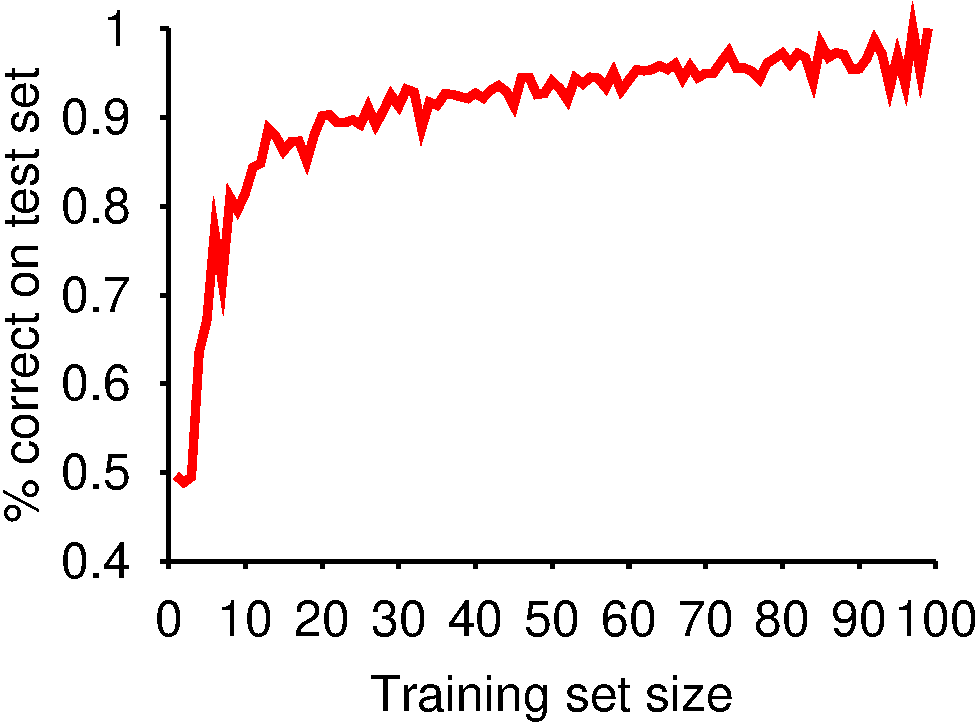
\includegraphics[height=2in]{restaurant-dtl-curve}
\end{center}
\end{frame}

\subsection{Overfitting and Underfitting}

\begin{frame}{Overfitting}
\begin{block}{Definition}
A hypothesis $h$ has \alert{overfit} the data if it uses a function that is more complex than necessary to explain the data
\end{block}
\smallskip
\begin{columns}[t]
\begin{column}<2->{1in}
Examples: \\
\medskip
$
\begin{array}{lll}
f(1) & = & 2 \\
f(2) & = & 4 \\
f(3) & = & 6 \\
\end{array}
$
\end{column}
\begin{column}<3->{3in}
Hypotheses: \\
\medskip
$
\begin{array}{lll}
h_1(x) & = & 2x \\
\uncover<4->{h_2(x) & = & \alert<5->{x^3 - 6x^2 + 13x - 6}} \\
\end{array}
$ \\
\medskip
\uncover<5->{$h_2$ has probably overfit the data} \\
\uncover<6->{\ldots\ unless $f(x) = x^3 - 6x^2 + 13x - 6$}
\end{column}
\end{columns}
\begin{block}<7->{Lesson}
Use as many parameters as we expect $f$ to have, no more
\end{block}
\end{frame}

\begin{frame}{Selecting Hypotheses}
\begin{columns}
\begin{column}{2.1in}
Many hypotheses possible:\\
\bigskip
\only<1>{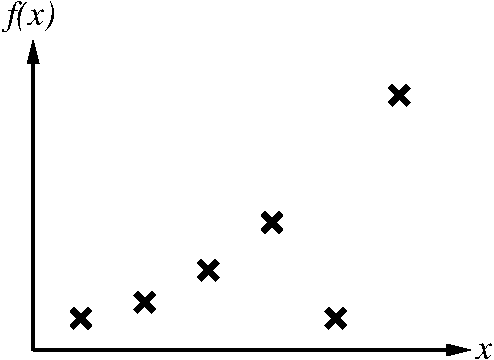
\includegraphics[height=1.5in]{curve-fitting-1}}%
\only<2>{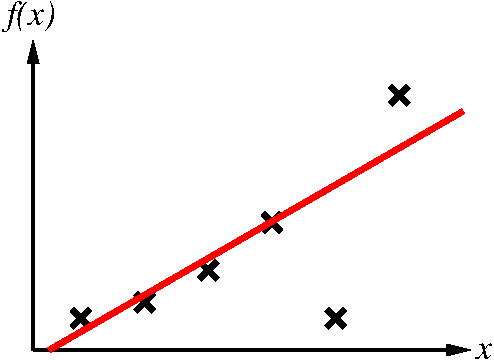
\includegraphics[height=1.5in]{curve-fitting-2}}%
\only<3>{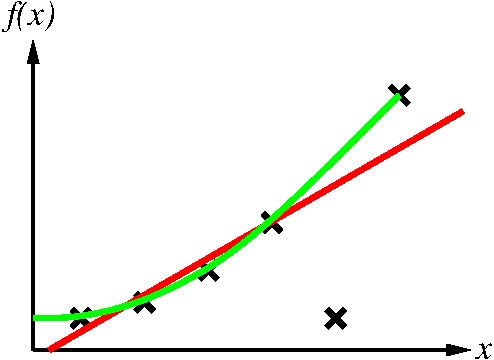
\includegraphics[height=1.5in]{curve-fitting-3}}%
\only<4>{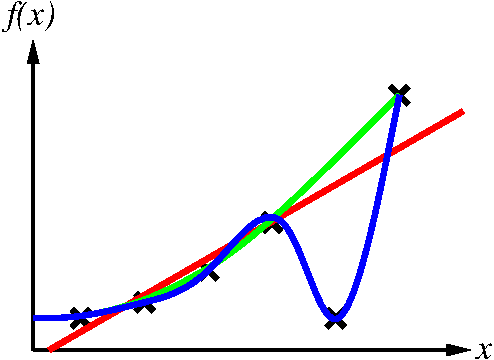
\includegraphics[height=1.5in]{curve-fitting-4}}%
\only<5->{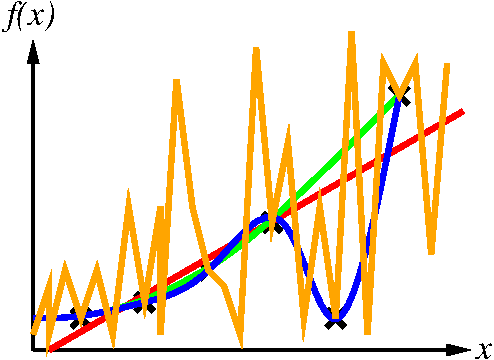
\includegraphics[height=1.5in]{curve-fitting-5}}%
\end{column}
\begin{column}<6->{2.1in}
\begin{block}{Goals}
\begin{itemize}
\item Maximize number of examples where $h$ agrees with $f$
\item Minimize complexity of $h$ function
\end{itemize}
\end{block}
\bigskip
\uncover<7->{Typically a tradeoff between consistency and simplicity}
\end{column}
\end{columns}
\end{frame}

\section{Supervised Learning Algorithms}

\begin{frame}{Learning Supervised Models}
After problem formulation, we apply a \alert{learning algorithm} \\
\medskip
\begin{block}{Input}
A set of $(x, f(x))$ training examples
\end{block}
\pause
\begin{block}{Output}
A function $h\!: D_f \rightarrow R_f$
\end{block}
\pause
\begin{block}{Goal}
Pick an $h$ that:
\begin{itemize}
\item is consistent with the training examples
\item does not overfit the data (i.e. is not overly complex)
\end{itemize}
\end{block}
\end{frame}


\subsection{Decision Trees}

\begin{frame}{Decision Trees}
\begin{columns}
\begin{column}{2.7in}
\centering
Should I play golf today? \\
\bigskip
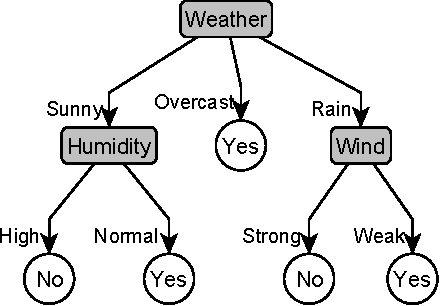
\includegraphics[width=2.7in]{play_golf}
\end{column}
\begin{column}{1.5in}
\begin{block}{Function}
$D_f$ = days \\
$R_f$ = $\{\textit{Yes}, \textit{No}\}$
\end{block}
\bigskip
\begin{block}{Features}
\begin{itemize}
\item Weather
\item Humidity
\item Wind
\end{itemize}
\end{block}
\end{column}
\end{columns}
\end{frame}

\begin{frame}{Decision Trees as Functions}
\begin{columns}[t]
\begin{column}{2in}
$f(X, Y) = X \textit{ xor } Y$ \\[1em]
\includegraphics[scale=.75]{xor}
\end{column}
\begin{column}{2in}
$f(A, B, C) = (A \land B) \lor \lnot C$ \\[1em]
\includegraphics[scale=.75]{abc}
\end{column}
\end{columns}
\end{frame}

\begin{frame}{Learning Decision Trees}
\begin{enumerate}
\item Select a feature $F$ for the node
\item For each value of $F$, create a child node
\item Sort training examples into child nodes
\item If examples are sorted perfectly, terminate
\item Else, repeat the process for each child node
\end{enumerate}
\begin{columns}
\begin{column}<2->{1.7in}
$
\begin{array}{cc|c}
X          &  Y          & f(X, Y) \\
\hline
\textit{true}  & \textit{true}   & \textit{true} \\
\textit{true}  & \textit{false}  & \textit{false} \\
\textit{false} & \textit{true}   & \textit{true} \\
\textit{false} & \textit{false}  & \textit{true} \\
\end{array}
$
\end{column}
\begin{column}{2.6in}
\only<-2>{\invisible{\includegraphics[scale=.75]{impl}}}%
\only<3>{\includegraphics[scale=.75]{impl-1}}%
\only<4>{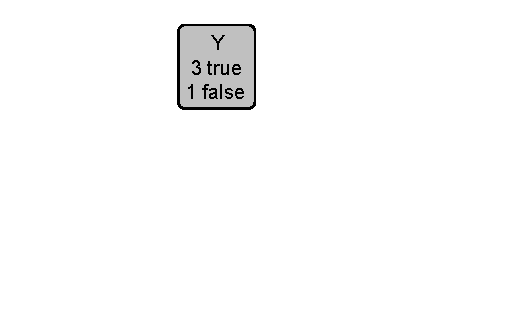
\includegraphics[scale=.75]{impl-2}}%
\only<5>{\includegraphics[scale=.75]{impl-3}}%
\only<6>{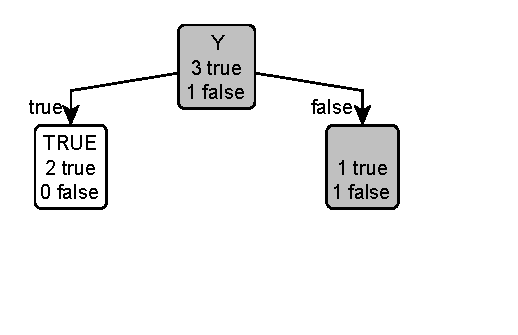
\includegraphics[scale=.75]{impl-4}}%
\only<7>{\includegraphics[scale=.75]{impl-5}}%
\only<8>{\includegraphics[scale=.75]{impl-6}}%
\only<9>{\includegraphics[scale=.75]{impl-7}}%
\end{column}
\end{columns}
\end{frame}

\begin{frame}[label=decision-tree-exercise]{Decision Tree Exercise}
\begin{columns}
\begin{column}{1.8in}
Build a decision tree for: \\
\bigskip
$
\begin{array}{ll|l}
F_1 & F_2 & \textit{Class} \\
\hline
0   & a   & \textit{true} \\
0   & b   & \textit{false} \\
1   & c   & \textit{true} \\
0   & c   & \textit{false} \\
1   & b   & \textit{false} \\
1   & a   & \textit{true} \\
\end{array}
$
\end{column}
\pause
\begin{column}{1.8in}
Two possible solutions: \\
\centering
\bigskip
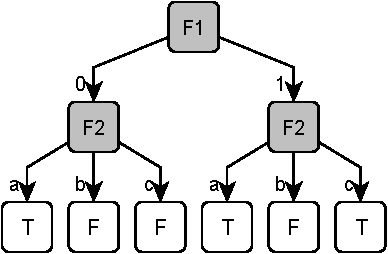
\includegraphics[scale=.6]{exercise-1} \\
\bigskip
\includegraphics[scale=.6]{exercise-2}
\end{column}
\end{columns}
\end{frame}

\begin{frame}{Selecting Features for Decision Trees}
\begin{block}{Feature Selection Order}
\begin{itemize}
\item Different orders result in different trees
\item ``Good'' features should be used before ``poor'' ones
\end{itemize}
\end{block}
\pause
\begin{block}{What is a ``good'' feature?}
One whose values predict the class labels \\
\end{block}
\pause
\medskip
\begin{columns}
\begin{column}{1.2in}
$
\begin{array}{lll}
F_1 & F_2 & \textit{Class} \\
\hline
a & 0 & \textit{true} \\
a & 1 & \textit{true} \\
b & 0 & \textit{false} \\
b & 1 & \textit{false} \\
\end{array}
$
\end{column}
\pause
\begin{column}{1.8in}
$F_1$ is a \alert{good} feature \\
\bigskip
$F_2$ is a \alert{poor} feature
\end{column}
\end{columns}
\end{frame}

\begin{frame}{Information}
\begin{block}{Good features provide more information}
Information can be quantified in terms of bits
\end{block}
\pause
Task: Encode \texttt{abacabad} using as few bits as possible
\pause
\medskip
\begin{columns}[t]
\begin{column}{1.8in}
Simple Encoding:
\begin{tabular}{ll}
a & 00 \\
b & 01 \\
c & 10 \\
d & 11 \\
\end{tabular} \\
\pause
\medskip
\texttt{abacabad} $\rightarrow$ 16 bits \texttt{0001001000010011}
\end{column}
\pause
\begin{column}{1.8in}
Using Probability:
\begin{tabular}{ll}
a & 0 \\
b & 10 \\
c & 110 \\
d & 111 \\
\end{tabular} \\
\pause
\medskip
\texttt{abacabad} $\rightarrow$ 14 bits \texttt{01001100100111}
\end{column}
\end{columns}
\pause
\bigskip
\alert{More likely values can be encoded in fewer bits!}
\end{frame}

\begin{frame}{Entropy}
\begin{block}{Definition}
The \alert{entropy} of a random variable $X$ is: \\
\smallskip
\tab\tab$H(X) = -\sum\limits_{x \in X}P(x)\log_2 P(x)$
\end{block}
\pause
\begin{block}{Bit-based Interpretation}
Smallest number of bits that can encode a stream of values from $X$'s distribution
\end{block}
\pause
\begin{block}{Intuitions}
\begin{itemize}
\item High entropy $\rightarrow$ boring (e.g. uniform) distribution
\item Low entropy $\rightarrow$ interesting distribution
\end{itemize}
\end{block}
\end{frame}

\begin{frame}{Entropy}
\begin{columns}
\begin{column}{1.1in}
\begin{tabular}{ll}
X       & Y   \\
\hline
math    & yes \\
history & no  \\
cs      & yes \\
math    & no  \\
math    & no  \\
cs      & yes \\
history & no  \\
math    & yes \\
\end{tabular}
\end{column}
\begin{column}{3.1in}
\pause
$
\extrarowheight=2pt
\begin{array}{lll}
H(X)        & = & \pause -\sum\limits_{x \in X}P(x)\log_2 P(x) \\
     \pause & = & -P(\textit{math})\log_2 P(\textit{math}) \\
            &   & -P(\textit{history})\log_2 P(\textit{history}) \\
            &   & -P(\textit{cs})\log_2 P(\textit{cs}) \\
     \pause & = & -\frac{1}{2}\log_2\frac{1}{2} 
                  -\frac{1}{4}\log_2\frac{1}{4}
                  -\frac{1}{4}\log_2\frac{1}{4} \\
     \pause & = & -\frac{1}{2}(-1) - \frac{1}{4}(-2) - \frac{1}{4}(-2) \\
     \pause & = & \frac{1}{2} + \frac{1}{2} + \frac{1}{2} \\
     \pause & = & 1.5 \\
\\
\pause
H(Y)        & = & \pause 1.0 \\
\end{array}
$
\end{column}
\end{columns}
\end{frame}

\begin{frame}{Specific Conditional Entropy}
\begin{columns}
\begin{column}{1.1in}
\begin{tabular}{ll}
X               & Y   \\
\hline
math            & yes \\
history         & no  \\
\alert<4-5>{cs} & \alert<4>{yes} \\
math            & no  \\
math            & no  \\
\alert<4-5>{cs} & \alert<4>{yes} \\
history         & no  \\
math            & yes \\
\end{tabular}
\end{column}
\begin{column}{3.1in}
\begin{block}{Specific Conditional Entropy}
$H(Y|X\!=\!x) = -\sum\limits_{y \in Y}P(y|x)\log_2 P(y|x)$
\end{block}
\small
$
\extrarowheight=2pt
\begin{array}{@{}l@{}l@{}l@{}}
\uncover<2->{H(Y|X\!=\!\textit{cs})}
& \uncover<2->{=}
& \uncover<3->{\alert<4>{-P(\textit{yes}|\textit{cs})\log_2 P(\textit{yes}|\textit{cs})}}
\\
&
& \uncover<3->{\alert<5>{-P(\textit{no}|\textit{cs})\log_2 P(\textit{no}|\textit{cs})}}
\\
& \uncover<4->{=}
& \uncover<4->{\alert<4>{-1 \log_2 1}}\uncover<5->{\alert<5>{-0 \log_2 0}}
\\
& \uncover<6->{=}
& \uncover<6->{-1 \cdot 0 - 0 \cdot \infty}
\\
& \uncover<7->{=}
& \uncover<7->{0} \\
\end{array}
$ \\
\medskip
\uncover<8->{In other words, $X\!=\!\textit{cs}$ is a great predictor of $Y$}
\end{column}
\end{columns}
\end{frame}

\begin{frame}{Conditional Entropy}
\begin{columns}
\begin{column}{1.1in}
\begin{tabular}{ll}
X               & Y   \\
\hline
math            & yes \\
history         & no  \\
cs              & yes \\
math            & no  \\
math            & no  \\
cs              & yes \\
history         & no  \\
math            & yes \\
\end{tabular}
\end{column}
\begin{column}{3.1in}
\begin{block}{Conditional Entropy}
$
\begin{array}{lll}
H(Y|X) & = & \sum\limits_{x \in X}P(X\!=\!x)H(Y|X\!=\!x)
\end{array}
$
\end{block}
\pause
\small
Given:
$
\begin{array}[t]{lll}
H(Y|X\!=\!\textit{math})    & = & 1 \\
H(Y|X\!=\!\textit{history}) & = & 0 \\
H(Y|X\!=\!\textit{cs})      & = & 0 \\
\end{array}
$ \\
\smallskip
\pause
$
\extrarowheight=2pt
\begin{array}{@{}l@{\hspace{2pt}}l@{\hspace{2pt}}l@{}}
H(Y|X) & = & \pause P(X\!=\!\textit{math}) H(Y|X\!=\!\textit{math}) + \mbox{}\\
       &   & P(X\!=\!\textit{history}) H(Y|X\!=\!\textit{history}) + \mbox{}\\
       &   & P(X\!=\!\textit{cs}) H(Y|X\!=\!\textit{cs}) \\
\pause & = & \frac{1}{2} \cdot 1 + \frac{1}{4} \cdot 0 + \frac{1}{4} \cdot 0 \pause = \frac{1}{2}
\end{array}
$ \\
\medskip
\pause
In other words, $X$ is a good predictor of $Y$
\end{column}
\end{columns}
\end{frame}

\begin{frame}{Information Gain}
\begin{columns}
\begin{column}{1.1in}
\begin{tabular}{ll}
X               & Y   \\
\hline
math            & yes \\
history         & no  \\
cs              & yes \\
math            & no  \\
math            & no  \\
cs              & yes \\
history         & no  \\
math            & yes \\
\end{tabular}
\end{column}
\begin{column}{3.1in}
\begin{block}{Information Gain}
$IG(Y|X) = H(Y) - H(Y|X)$
\end{block}
\pause
\begin{block}{Intuitive Explanation}
How many bits would it save to know $X$?
\end{block}
\pause
$
\begin{array}[t]{lll}
H(Y|X)  & = & 0.5 \\
H(Y)    & = & 1 \\
\\
\pause
IG(Y|X) & = & \pause 1 - 0.5 = 0.5
\end{array}
$
\end{column}
\end{columns}
\end{frame}

\begin{frame}{Decision Trees and Information Gain}
\textbf{\keyword{Select the feature with the highest information gain}}
\pause
\medskip
\begin{columns}[T]
\begin{column}{0.6in}
\small
$
\begin{array}{@{}l@{\hspace{2pt}}l@{\hspace{2pt}}|@{\hspace{2pt}}l@{}}
F_1 & F_2 & Y \\
\hline
0   & a   & \textsc{t} \\
0   & b   & \textsc{f} \\
1   & c   & \textsc{t} \\
0   & c   & \textsc{f} \\
1   & b   & \textsc{f} \\
1   & a   & \textsc{t} \\
\end{array}
$
\end{column}
\pause
\begin{column}{3.8in}
\small
$
\extrarowheight=2pt
\begin{array}{@{}l@{\hspace{2pt}}l@{\hspace{2pt}}l@{}}
H(Y)               & = & \pause -P(\textsc{t})\log_2 P(\textsc{t}) - P(\textsc{f})\log_2 P(\textsc{f}) \\
\pause
                   & = & -\frac{1}{2}\log_2 \frac{1}{2} - \frac{1}{2}\log_2 \frac{1}{2} \pause = 1 \\
\pause
H(Y|F_1\!\!=\!\!0) & = & \pause -P(\textsc{t}|0)\log_2 P(\textsc{t}|0) - \pause P(\textsc{f}|0)\log_2 P(\textsc{f}|0) \\
\pause
                   & = & - \frac{1}{3}\log_2 \frac{1}{3} - \pause \frac{2}{3}\log_2 \frac{2}{3} \pause = 0.92\\
\pause         
H(Y|F_1\!\!=\!\!1) & = & \pause \ldots = 0.92\\
\pause         
H(Y|F_1)           & = & \pause P(F_1\!\!=\!\!0) H(Y|F_1\!\!=\!\!0) + P(F_1\!\!=\!\!1) H(Y|F_1\!\!=\!\!1) \\
\pause         
                   & = & 0.5 \cdot 0.92 + \pause 0.5 \cdot 0.92 \pause = 0.92 \\
\pause
IG(Y|F_1)          & = & \pause H(Y) - H(Y|F_1) \pause = 1 - 0.92 \pause = 0.08 \\
\pause         
IG(Y|F_2)          & = & \pause \mbox{\alert{ Your turn! }} \pause = 0.67 \\
\end{array}
$ \\
\medskip
\pause
So $F_2$ is a much better feature to split on \hyperlink{decision-tree-exercise<2>}{\beamerbutton{See Example}}
\end{column}
\end{columns}
\end{frame}

\subsection{Random Forests}

\begin{frame}[<+->]{Random Forests}
\begin{block}{Key Ideas}
\begin{itemize}
\item Voting works better when classifiers are independent
\item Partially random trees should be more independent
\end{itemize}
\end{block}
\begin{block}{Random Forests}
\begin{enumerate}
\item\label{sample-step} Generate a bootstrap sample of $n$ examples
\item\label{select-step} For each node, select $k$ features at random
\item\label{split-step} Split on the feature with the highest information gain
\item Repeat steps \ref{sample-step}, \ref{select-step} and \ref{split-step} to generate $n$ decision trees
\item Classify by taking the majority vote
\end{enumerate}
\end{block}
\end{frame}

\begin{frame}{Random Forest Exercise}
\begin{columns}
\begin{column}{1.2in}
\small
$
\begin{array}{lll|l}
F_0 & F_1 & F_2 & C \\
\hline
0   & 0   & 0   & F \\
0   & 0   & 1   & F \\
0   & 1   & 1   & F \\
1   & 0   & 1   & F \\
1   & 0   & 0   & T \\
1   & 1   & 1   & T \\
\end{array}
$
\end{column}
\begin{column}{2.8in}
\begin{itemize}
\item Generate a bootstrap sample
\item Example indices $[0, 5, 0, 1, 5, 4]$
\item Generate a random decision tree
\item Feature indices $[1, 2]$ then $[2, 0]$
\end{itemize}
\end{column}
\end{columns}
\pause
\begin{columns}
\begin{column}{1.2in}
\small
$
\begin{array}{lll|l}
F_0 & F_1 & F_2 & C \\
\hline
0   & 0   & 0   & F \\
1   & 1   & 1   & T \\
0   & 0   & 0   & F \\
0   & 0   & 1   & F \\
1   & 1   & 1   & T \\
1   & 0   & 0   & T \\
\end{array}
$
\end{column}
\begin{column}{2.8in}
\includegraphics[width=2in]{random-tree}
\end{column}
\end{columns}
\end{frame}

\begin{frame}[<+->]{Random Forest Properties}
\begin{block}{Disadvantages}
\begin{itemize}
\item Hard to estimate complexity due to random factor
\item $k$ (\# of features) must be determined experimentally
\end{itemize}
\end{block}
\begin{block}{Advantages}
\begin{itemize}
\item State of the art performance on many datasets
\item Relatively simple to implement
\item Expected error can be determined while training
\begin{itemize}
\item Bootstrap sample leaves out about $\frac{1}{3}$ of examples
\item Use these out-of-bag examples to test individual trees
\item Collect votes from all trees to get overall accuracy
\end{itemize}
\end{itemize}
\end{block}
\end{frame}

\part{Key Ideas}

\begin{frame}{Key Ideas}
\begin{block}{Supervised Learning}
\begin{itemize}
\item Input: $(x, f(x))$ examples
\item Output: $h$, a guess at $f$
\item Domain objects usually decomposed into features
\end{itemize}
\end{block}
\begin{block}{Decision Trees}
\begin{itemize}
\item Each node splits examples by feature values
\item Best feature yields the highest information gain
\item Bagging, boosting and random forests combine trees
\end{itemize}
\end{block}
\end{frame}

\end{document}


